\documentclass[12pt, oneside, openany]{book}

\usepackage{mathptmx} % Contiene una fuente similar a Times New Roman

\usepackage[spanish, es-tabla]{babel} % Permite escritura en castellano
\usepackage[utf8]{inputenc} % Permite utilizar caracteres UTF8

\usepackage{graphicx} % Para la inclusión de gráficos e imágenes
\graphicspath{ {images/} } % Ruta para buscar las imágenes
\usepackage[a4paper,top=30mm,left=30mm,right=25mm,bottom=25mm,headheight=20mm]{geometry} % Configuración de los margenes de la página

% Paquetes para que funcione el formato.
\usepackage{titlesec}
\usepackage{setspace}
\usepackage{ragged2e}
\usepackage{fancyhdr}
\usepackage{lastpage}
\usepackage{stackengine}
\usepackage{array}
\usepackage[hidelinks]{hyperref}
\usepackage{enumitem}
\usepackage{float}
\usepackage{hypcap}
\usepackage{caption}
\usepackage{fancyvrb}
\usepackage{amsfonts}
\usepackage{tabularx}
\usepackage{multirow}

\usepackage{hyperref} % Paquete para que las referencias funcionen, y permite introducir links
\usepackage[table]{xcolor} % Paquete para trabajar con colores (fondo de celdas, color del texto...)
% Se define un color gris desde su código RGB
\definecolor{gris}{RGB}{220,220,220}

\setcounter{secnumdepth}{3} % Para permitir numerar las sub-subsecciones

% Modifica el nombre de los índices al castellano
\addto\captionsspanish{
  \renewcommand{\contentsname}{Índice de contenido}
  \renewcommand{\listfigurename}{Índice de figuras}
  \renewcommand{\listtablename}{Índice de tablas}
}

% Formateo de los nombres de los apartados:
\titleformat{\chapter}[block]
  {\normalfont\Huge\bfseries\singlespacing}{\thechapter.}{1em}{\Huge}
\titlespacing*{\chapter}{0pt}{-62pt}{0pt}

\titleformat{\section}[block]
  {\normalfont\Large\bfseries}{\thesection.}{4pt}{\Large}
\titlespacing*{\section}{0pt}{\baselineskip}{0pt}

\titleformat{\subsection}[block]
  {\normalfont\large\bfseries}{\thesubsection.}{4pt}{\normalsize\large}
\titlespacing*{\subsection}{0pt}{0pt}{0pt}

\titleformat{\subsubsection}[block]
  {\normalfont\normalsize\bfseries}{\thesubsubsection.}{4pt}{\normalsize}
\titlespacing*{\subsubsection}{0pt}{0pt}{0pt}

\def\tablename{Tabla}

%% Variables para portada y cabeceras
%% Cambiar los valores para cada documento!!!
\def\title{Ejercicio Teórico 1}
\def\subject{Pruebas y Despliegue de Software}
\def\author{Juan Francisco Mier Montoto}
\def\target{www.mier.info}
\def\authorid{UO283319}
\def\date{marzo 2024}
\def\org{Escuela Politécnica de Ingeniería de Gijón}
\def\area{Grado en Ingeniería Informática en Tecnologías de la Información}

\def\ORG{\expandafter\MakeUppercase\expandafter{\org}}
\def\AREA{\expandafter\MakeUppercase\expandafter{\area}}
\def\SUBJECT{\expandafter\MakeUppercase\expandafter{\subject}}

\captionsetup{justification=centering}
\setlength{\headheight}{65pt}

\fancyhf{}
\fancyhead[L]{
\includegraphics[height=16mm]{style/square.png}
  \hspace{1em} \Longstack[l] {
    \textbf{\SUBJECT} \newline
    \textbf{\title}}
  \newline \leftmark{}
}
\fancyhead[R]{\bfseries{Hoja \hyperlink{toc}{\thepage}~de~\pageref{LastPage}}}
\fancyfoot[C]{\href{\target}{\author}}
\renewcommand{\headrulewidth}{0pt} % default is 0pt
\renewcommand{\footrulewidth}{0.4pt} % default is 0

\fancypagestyle{plain}{%
  \fancyhf{}
  \fancyhead[L]{
\includegraphics[height=16mm]{style/square.png}
    \hspace{1em} \Longstack[l]{
      \textbf{\SUBJECT} \newline
      \textbf{\title}}}
  \fancyhead[R]{\bfseries{Hoja \hyperlink{toc}{\thepage}~de~\pageref{LastPage}}}
  \fancyfoot[C]{\href{\target}{\author}}
  \renewcommand{\headrulewidth}{0pt} % default is 0pt
  \renewcommand{\footrulewidth}{0.4pt} % default is 0pt
}

\pagestyle{fancy}

\restylefloat{table}



\begin{document}

\rmfamily % Fuente tipo Romana

% Portada de la memoria
\begin{titlepage}
    \centering
    \bfseries {
        \null{}
        \vspace{0cm}
        \begin{table}[h]
            \centering
            \begin{tabular}{m{10cm} m{1cm} m{3cm}}
                \vspace{0.2cm}
                
\includegraphics[width=86mm]{style/full.png} &  & \vspace{1.52mm} 
\includegraphics[width=23mm]{style/square.png} \\
            \end{tabular}
        \end{table}

        \vspace{3\baselineskip}

        \Large{\ORG{} \\ \vspace{3\baselineskip}}
        \large {
            \AREA{} \\ \vspace{3\baselineskip}
            \subject{} \\ \vspace{2\baselineskip}

            % TRABAJO FIN DE GRADO/MÁSTER Nº XXXXXXXXX \vspace{\baselineskip} \\
            \title{} \\ \vspace{3\baselineskip}

            \author{} \\
            \authorid{} \\
            % TUTOR/ES: \\
            % D. APELLIDO1 APELLIDO2, Nombre \\
            % D. APELLIDO1 APELLIDO2, Nombre \\  \vspace{\baselineskip}

            \vspace{2\baselineskip}
            FECHA:\@ \date{}
        }
    }
\end{titlepage}


% Índice de contenido
\addcontentsline{toc}{chapter}{Índice de contenido} % Añade la referencia al índice de contenido
\hypertarget{toc}{}
\tableofcontents
\newpage{}

% Índice de figuras
\addcontentsline{toc}{chapter}{Índice de figuras}  % Añade la referencia al índice de contenido
\hypertarget{lof}{}
\listoffigures

\justify{} % Texto justificado
\setlength{\parskip}{\baselineskip} % Separación entre párrafos de 1 linea
\onehalfspacing{}

%% El contenido de la memoria, dividido en capítulos:
\chapter{Introducción}


\input{sections/2_diseño.tex}
\chapter{Análisis de valores límite}
Para el análisis de valores límite, se han seleccionado los valores límite de las clases de equivalencia
de entrada definidas en el capítulo anterior, poniendo especial atención al cumplimiento de las aperturas
de los intervalos.

\section{Base imponible ($BI$)}
Debido a la naturaleza de esta variable, se han seleccionado los valores límite de los intervalos definidos
anteriormente.
\begin{itemize}
	\item $BI = 0$€
	\item $BI = 8999$€
	\item $BI = 9000$€
	\item $BI = 12449$€
	\item $BI = 12450$€
	\item $BI = 20199$€
	\item $BI = 20200$€
	\item $BI = 35199$€
	\item $BI = 35200$€
	\item $BI = 59999$€
	\item $BI = 60000$€
	\item $BI = 299999$€
	\item $BI = 300000$€
\end{itemize}
\newpage{}
\section{Retenciones ($R$)}
Esta variable es especialmente interesante para el AVL, ya que el cálculo de las retenciones depende
directamente de la base imponible, por lo que debería haber una relación directa entre los valores límite
de ambas variables.
\begin{itemize}
	\item $R = 0$€
	\item $R = BI - 1$€
	\item $R = BI$€
	\item $R = BI + 1$€
\end{itemize}

\section{Número de empleadores}
En esta sección no se considera relevante aplicar técnicas AVL, ya que el mero cumplimiento de las
diferentes clases de equivalencia garantiza el correcto funcionamiento del sistema debido a la pertenencia de
los posibles valores al conjunto entero.

\section{Préstamos hipotecarios}
Puesto que al resultado del cálculo de los impuestos se le aplican las deducciones correspondientes
(en este enunciado solo se considera esta), los valores límite de esta variable solo afectan al
hecho de si se aplica o no la deducción en sí, sin tener en cuenta el efecto de la deducción en el
cálculo final. Para una comprobación más exhaustiva, se deberían considerar valores exactos que
modifiquen el resultado final del cálculo de los impuestos teniendo en cuenta dichas deducciones.

Puesto a que, como se indica en el diseño, la deducción no tiene un punto de corte ($9040$€), sino que
se trata de un valor máximo, el valor del préstamo hipotecario no se considera relevante para el
planteamiento de los casos de prueba ya que tampoco se calcula el valor de la deducción para las pruebas.

\chapter{Casos de prueba}
\section{Tabla de casos}
\begin{table}[H]
	\centering
	\captionof{figure}{Casos de prueba iniciales propuestos para el sistema}
	\begin{tabular}{l|c c c|r r r}
		\hline
		\multirow{2}*{\bf{ID}} & \multicolumn{3}{c|}{\textbf{Entradas}} & \multicolumn{3}{c}{\bf{Salidas}} \\
		\cline{2-7}
		& $BI$ & $R$ & $n_{E}$ & Obligatoriedad & Máx. grav. & Resultado \\
		\hline
		\hline
		CP1 & 0€ & 0€ & 0 & No & 19\% & Sin cambios \\
		CP2 & 8999€ & 0€ & 1 & No & 19\% & A pagar \\
		CP3 & 8999€ & 0€ & 2 & Sí & 19\% & A pagar \\
		CP4 & 9000€ & 0€ & 1 & Sí & 19\% & A pagar \\
		CP5 & 12449€ & $I-1$€ & 1 & Sí & 19\% & A pagar \\
		CP6 & 12450€ & $I+1$€ & 1 & Sí & 19\% & A devolver \\
		CP7 & 20199€ & $I$€ & 1 & Sí & 19\% & Sin cambios \\
		CP8 & 20200€ & 0€ & 1 & Sí & 30\% & A pagar \\
		CP9 & 35199€ & 0€ & 1 & Sí & 30\% & A pagar \\
		CP10 & 35200€ & 0€ & 1 & Sí & 37\% & A pagar \\
		CP11 & 59999€ & 0€ & 1 & Sí & 37\% & A pagar \\
		CP12 & 60000€ & 0€ & 1 & Sí & 45\% & A pagar \\
		CP13 & 299999€ & 0€ & 1 & Sí & 45\% & A pagar \\
		CP14 & 300000€ & 0€ & 1 & Sí & 47\% & A pagar \\
		\hline
	\end{tabular}
\end{table}

Los anteriores casos de prueba no cubren situaciones de validación de datos ya que no se considera relevante
para este entregable teórico, para ello se definen algunos breves ejemplos de validación de datos:
\begin{table}[H]
	\centering
	\captionof{figure}{Ejemplos de casos de prueba de validación de datos}
	\begin{tabular}{l|c c c|r r r}
		\hline
		\multirow{2}*{\bf{ID}} & \multicolumn{3}{c|}{\textbf{Entradas}} & \multicolumn{3}{c}{\bf{Salidas}} \\
		\cline{2-7}
		& $BI$ & $R$ & $n_{E}$ & Obligatoriedad & Máx. grav. & Resultado \\
		\hline
		\hline
		CP20 & -1€ & 0€ & 1 & \multicolumn{3}{c}{Error\cellcolor{red!25}} \\
		CP21 & 0€ & -1€ & 1 & \multicolumn{3}{c}{Error\cellcolor{red!25}} \\
		CP22 & 0€ & 0€ & -1 & \multicolumn{3}{c}{Error\cellcolor{red!25}} \\
		\hline
	\end{tabular}
\end{table}

\section{Trazabilidad}
\begin{minipage}{\linewidth}
	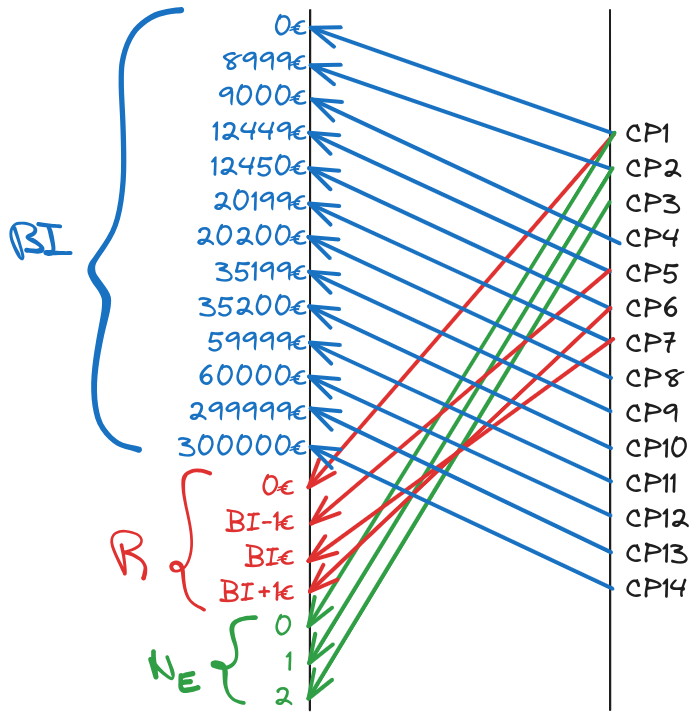
\includegraphics[width=\textwidth]{trazabilidad.png}
	\captionof{figure}{Trazabilidad del sistema}
\end{minipage}

\chapter{Combinatioria}
\section{Árbol de combinación}
A continuación, se muestra un ejemplo de árbol de combinación que utiliza la técnica
\textit{Base Choice} para el cálculo de las combinaciones posibles de un sistema de
tres variables de entrada, en este caso $BI$, $R$ y $n_{E}$.

\begin{minipage}{\linewidth}
	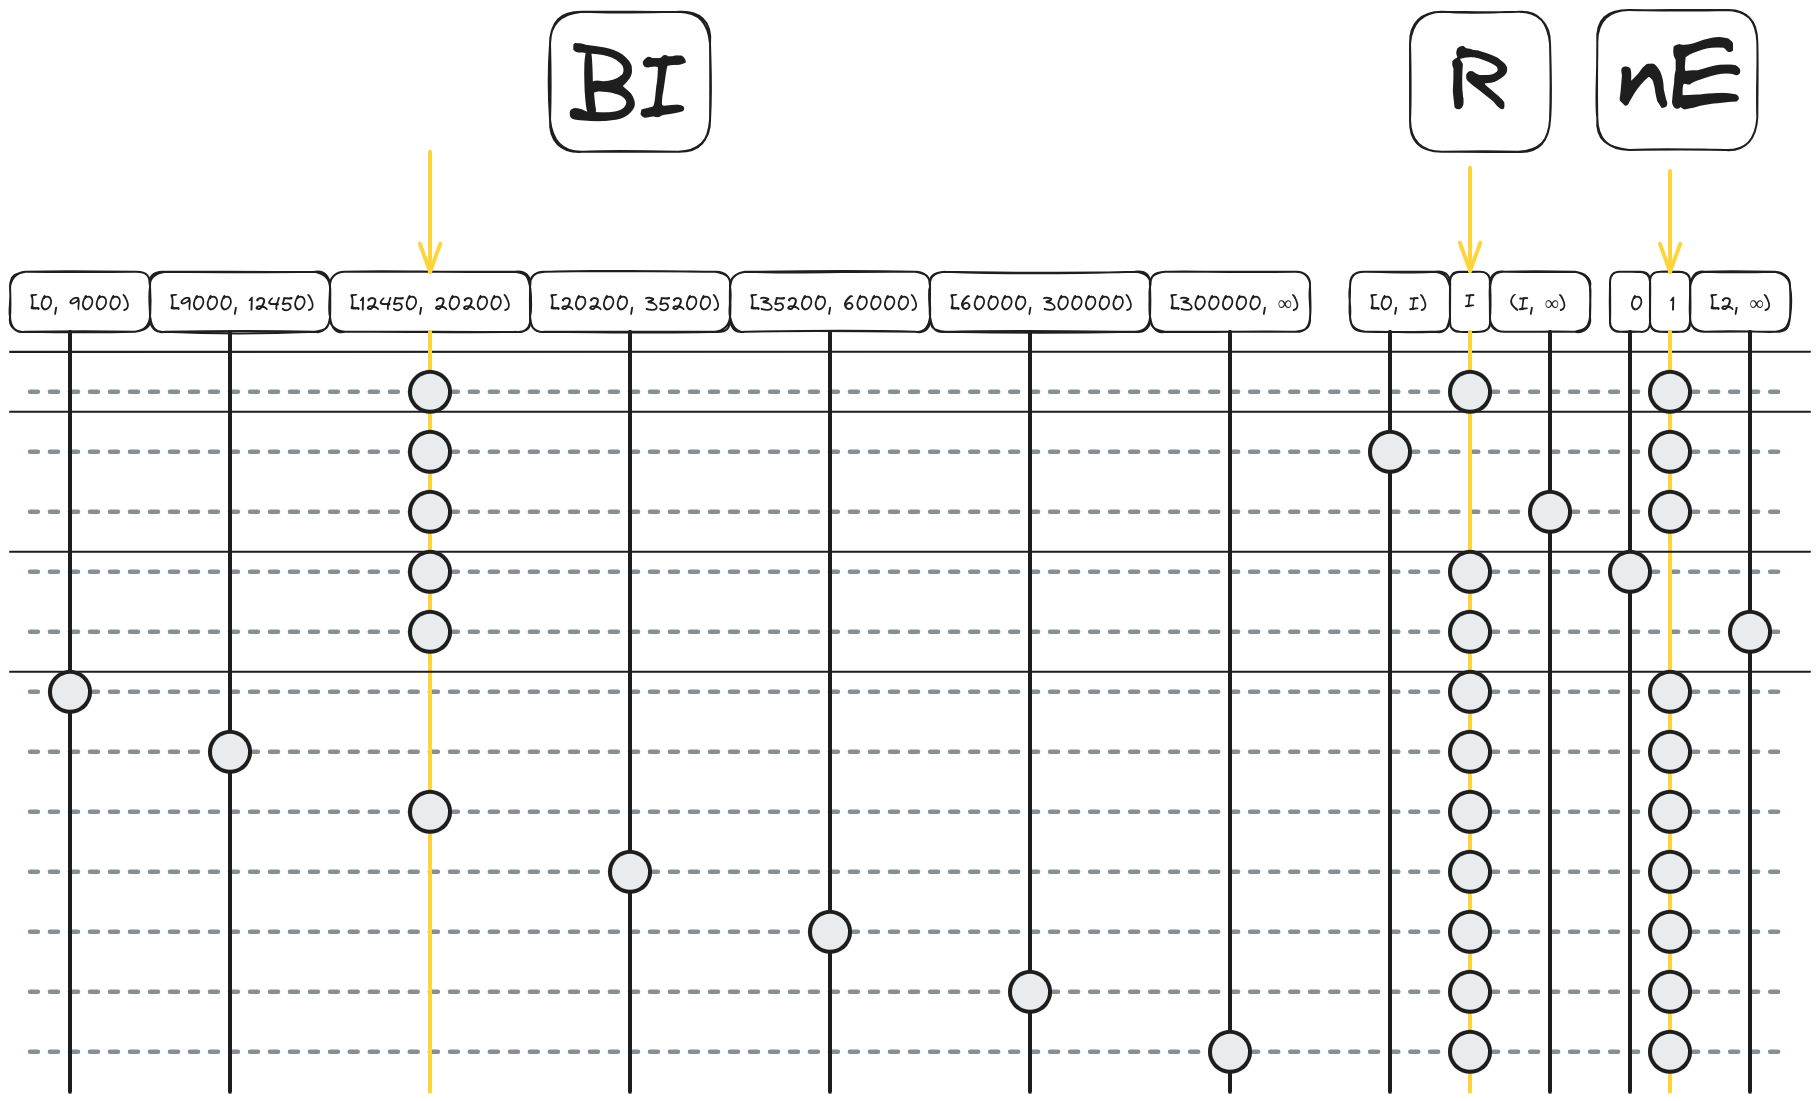
\includegraphics[width=\textwidth]{arbol.png}
	\captionof{figure}{Árbol de decisiones \textit{base choice} con tres variables}
\end{minipage}

En el diagrama anterior, se resaltan los casos seleccionados como ``base'' en amarillo.

\section{Ejemplo de caso de prueba}
A continuación, se muestra un ejemplo de caso de prueba del árbol anterior (último caso
de la variación de la variable $n_{E}$).
\begin{table}[H]
	\centering
	\captionof{figure}{Ejemplo de caso de prueba de combinación}
	\begin{tabular}{l|c c c|r r r}
		\hline
		\multirow{2}*{\bf{ID}} & \multicolumn{3}{c|}{\textbf{Entradas}} & \multicolumn{3}{c}{\bf{Salidas}} \\
		\cline{2-7}
		& $BI$ & $R$ & $n_{E}$ & Obligatoriedad & Máx. grav. & Resultado \\
		\hline
		\hline
		CP99 & 20000€ & $I$€ & 3 & Sí & 24\% & Sin cambios \\
		\hline
	\end{tabular}
\end{table}

\chapter{Preguntas del enunciado (ejercicio 5)}
\section{Posibles consecuencias ante un fallo}
El fallo de un software de estas características, ya sea por un error en el cálculo de los impuestos, caída
del servicio o cualquier otro problema que afecte al funcionamiento del sistema, puede tener consecuencias
catastróficas para los ciudadanos, ya que el cálculo de los impuestos es un proceso que afecta directamente
a la economía tanto del individuo como del estado.

En caso de fallo, la ciudadanía podría verse afectada por sanciones económicas por parte de la administración
sin justificación ninguna o incluso por la pérdida de dinero en concepto de impuestos que no se deberían haber
pagado. Por otro lado, el estado podría verse afectado por la pérdida de ingresos en concepto de impuestos que
no se han cobrado, lo que podría afectar a la economía del país.

\section{Noticias relevantes}
El fallo de software relacionado con administraciones públicas no es ficción, y de hecho es
más que frecuente. A continuación se citan algunas noticias que dejan en evidencia este hecho:
\begin{itemize}
	\item <<El 61\% de los usuarios han tenido problemas al usar las webs o apps de administraciones públicas>> \cite{newtral}
	\item <<Fallos en los programas y sistemas caídos: programas desactualizados lastran la actividad en Empleo>> \cite{abc}
	\item <<Sigue sin funcionar>> \cite{elpais}
\end{itemize}


%% Esto incluirá la bibliografía correctamente en nuestro trabajo
\newpage % En una nueva página
\addcontentsline{toc}{chapter}{Bibliografía} % Añade la referencia al índice de contenido

\bibliographystyle{ieeetr} % Define el estilo de la bibliografía
\bibliography{biblio} % Indica el archivo que contiene la colección de citas

\nocite{template}
\nocite{sumup}

\end{document}
